\documentclass{article}
\usepackage[utf8]{inputenc}
\usepackage{amsmath}
\usepackage{listings}
\usepackage{graphicx}
\usepackage[shortlabels]{enumitem}

\title{CIS 419/519: Homework 1}
\author{Your name here}
\date{}

\begin{document}
    \maketitle
    Although the solutions are my own, I consulted with the following people while working on this homework: \{Names here\}

    \begin{enumerate}
        \item % 1
        \begin{enumerate}
            \item % a
            Show your work:
            \begin{equation*}
                P(\textrm{play outside = yes}) =
            \end{equation*}
            \begin{equation*}
                P(\textrm{play outside = no}) =
            \end{equation*}
            ...
            \begin{equation*}
                IG_{Snow} =
            \end{equation*}
            \begin{equation*}
                IG_{Sunny} =
            \end{equation*}
            Snow/Sunny is better because...

            \item % b
            % The template tree is meaningless (it's not a hint about what the answer is)
            \begin{verbatim}
                if color = blue:
                  if size = small:
                    if act = stretch:
                      inflated = T
            \end{verbatim}

            \item % c
            Yes/No because...
        \end{enumerate}

        \item % 2
        \begin{enumerate}
            \item % (a)
            See Figure~\ref{fig:model_performance} for the model performance in the Madelon dataset. (The figure was generated on a different dataset, so replace the \texttt{plot.png} file with your own.)
            \begin{figure}
                \centering
                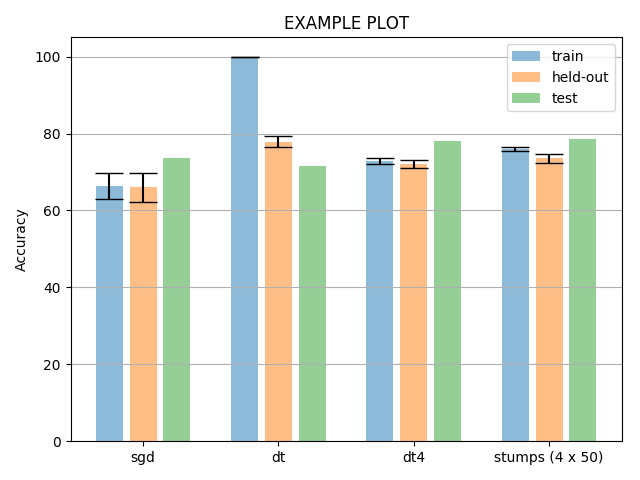
\includegraphics[width=\textwidth]{plot.png}
                \caption{Model performance on the Madelon dataset}
                \label{fig:model_performance}
            \end{figure}

            \begin{enumerate}[1.]
                \item
                \item
                \item
                \item
            \end{enumerate}

            \item % (b)
            The models' accuracies on the Badges dataset were as follows:
            \begin{center}
                \begin{tabular}{|c|c|}
                    \hline
                    Algorithm & Accuracy \\
                    \hline
                    SGD & a \\
                    Decision Tree & b \\
                    Decision Stump & c \\
                    SGD + Decision Stump Features & d \\
                    \hline
                \end{tabular}
            \end{center}

            \begin{enumerate}[1.]
                \item
            \end{enumerate}

            For extra credit, I did ...
        \end{enumerate}
    \end{enumerate}
\end{document}
